\documentclass[a4paper,12pt]{article}
\usepackage[utf8]{inputenc}
\usepackage[spanish]{babel}
\usepackage{color}
\usepackage{parskip}
\usepackage{graphicx}
\usepackage{multirow}
\usepackage{listings}
\usepackage{vmargin}
\usepackage{datetime}
\newdate{date}{2}{11}{2017}
\graphicspath{ {imagenes/} }
\definecolor{mygreen}{rgb}{0,0.6,0}
\definecolor{lbcolor}{rgb}{0.9,0.9,0.9}
\usepackage{epstopdf}
\usepackage{float}


\setpapersize{A4}
\setmargins{2.5cm}       % margen izquierdo
{1.5cm}                        % margen superior
{16.5cm}                      % anchura del texto
{23.42cm}                    % altura del texto
{10pt}                           % altura de los encabezados
{1cm}                           % espacio entre el texto y los encabezados
{0pt}                             % altura del pie de página
{2cm}     

\lstset{
    tabsize=4,    
%   rulecolor=,
    language=[GNU]C++,
        basicstyle=\tiny,
        aboveskip={1.5\baselineskip},
        columns=fixed,
        showstringspaces=false,
        extendedchars=false,
        breaklines=true,
        prebreak = \raisebox{0ex}[0ex][0ex]{\ensuremath{\hookleftarrow}},
        frame=single,
        showtabs=false,
        showspaces=false,
        showstringspaces=false,
        identifierstyle=\ttfamily,
        keywordstyle=\color[rgb]{0,0,1},
        commentstyle=\color[rgb]{0.026,0.112,0.095},
        stringstyle=\color{red},
        numberstyle=\color[rgb]{0.205, 0.142, 0.73},
%        \lstdefinestyle{C++}{language=C++,style=numbers}’.
}


\begin{document}
\title{Ejercicio de Dibujos}
\author{
Christofer Fabián Chávez Carazas \\
\small{Universidad Nacional de San Agustín de Arequipa} \\
\small{Escuela Profesional de Ciencia de la Computación} \\
\small{Computación Gráfica}
}
\date{\displaydate{date}}

\maketitle

Las primitivas usadas en los dibujos de los ejercicios están en los archivos \textit{primitivas.h} y \textit{matrix.h}

\begin{itemize}
 \item \textbf{matrix.h}
 
 En este archivo está la clase Matrix, usada para guardar el borde de una figura, línea o curva. También es usado para pintar un polígono.
 
 \begin{lstlisting}
#ifndef MATRIX_H
#define MATRIX_H

#include <GL/glut.h>
#include <iostream>
#include <algorithm>
#include <cmath>

using namespace std;

struct Window{
    int width;
    int height;
};


class Matrix{
public:
    Matrix(){};
    Matrix(Window window);
    Matrix operator+(Matrix b);

    bool ** matrix;
    Window size;
    GLint yMax;
    GLint yMin;
    GLint xMax;
    GLint xMin;
};


Matrix::Matrix(Window window){
    size = window;
    matrix = new bool*[window.height];
    for(int i = 0; i < window.height; i++){
        matrix[i] = new bool[window.width];
        for(int j = 0; j < window.width; j++){
            matrix[i][j] = 0;
        }
    }
}

Matrix Matrix::operator+(Matrix b){
    for(int i = this->yMax; i >= this->yMin; i--){
        int y = abs(i - this->size.height - 1);
        for(int j = this->xMin; j <= this->xMax; j++){
            if(this->matrix[y][j] == 1) b.matrix[y][j] = 1;
        }
    }
    b.xMax = max(this->xMax,b.xMax);
    b.xMin = min(this->xMin,b.xMin);
    b.yMax = max(this->yMax,b.yMax);
    b.yMin = min(this->yMin,b.yMin);
    return b;
}

#endif
 \end{lstlisting}

 \item \textbf{primitivas.h}

Aquí se encuentran las funciones \textit{DDA} (líneas), \textit{bresenham} (líneas), \textit{drawLineXnpio} (función para dibujar líneas hecha por mí en otra práctica),
\textit{circleMidPoint} (círculos), \textit{elipceMidPoint} (elipses), \textit{bezier}  (curvas), \textit{fillFigure} (pintar figura).
 
\begin{lstlisting}
#ifndef PRIMITIVAS_H
#define PRIMITIVAS_H

#include <GL/glut.h>
#include <iostream>
#include <cmath>
#include <algorithm>
#include <vector>
#include <tuple>
#include "matrix.h"

using namespace std;

enum COLORES {ROJO,AZUL,VERDE,NEGRO,BLANCO};
enum Direcciones {ARRIBA,ABAJO,DERECHA,IZQUIERDA};


struct Point{
    GLint x;
    GLint y;
};

void drawLine(Point a, Point b){
    glBegin(GL_LINES);
        glVertex2i(a.x, a.y);
        glVertex2i(b.x, b.y);
    glEnd();
}


void drawPoint(Point p){
    glBegin(GL_POINTS);
        glVertex2i(p.x, p.y);
    glEnd();
}

void setPixel(GLint x, GLint y){
    glBegin(GL_POINTS);
        glVertex2i(x,y);
    glEnd();
}

void setPixel(GLint x, GLint y, Matrix &resMatrix){
    if(y < resMatrix.size.height and x < resMatrix.size.width){
        resMatrix.matrix[abs(y - resMatrix.size.height - 1)][x] = 1;
    }
    glBegin(GL_POINTS);
        glVertex2i(x,y);
    glEnd();
}

tuple<int,int> getDir(int x1, int y1, int x2, int y2){
    int dirX = -1;
    int dirY = -1;
    if(x1 < x2) dirX = DERECHA;
    else dirX = IZQUIERDA;
    if(y1 < y2) dirY = ARRIBA;
    else dirY = ABAJO;
    return make_tuple(dirX,dirY);
}

Matrix drawLineXnpio(Point ini, Point fin, Window window){
    int x1 = ini.x;
    int y1 = ini.y;
    int x2 = fin.x;
    int y2 = fin.y;

    Matrix resMatrix(window);
    resMatrix.yMin = min(y1,y2);
    resMatrix.yMax = max(y1,y2);
    resMatrix.xMax = max(x1,x2);
    resMatrix.xMin = min(x1,x2);

    if(x1 == x2){
        int yMin = min(y1,y2);
        int yMax = max(y1,y2);

        for(int i = yMin; i <= yMax; i++){
            setPixel(x1,i,resMatrix);
        }
    }
    else if(y1 == y2){
        int xMin = min(x1,x2);
        int xMax = max(x1,x2);
        for(int i = xMin; i <= xMax; i++){
            setPixel(i,y1,resMatrix);
        }
    }
    else{
        int dirX = -1;
        int dirY = -1;
        tie(dirX,dirY) = getDir(x1,y1,x2,y2);
        int ejeMax = max(abs(x1-x2) + 1,abs(y1-y2) + 1);
        int ejeMin = min(abs(x1-x2) + 1,abs(y1-y2) + 1);
        float saltosF = (float)ejeMax / (float)ejeMin;
        int saltos = saltosF;
        float decimalesSaltos = saltosF - saltos;
        float decimalActual = 0;
        int direcX = 1;
        int direcY = 1;
        int actualX = x1;
        int actualY = y1;
        if(dirX == IZQUIERDA) direcX = -1;
        if(dirY == ABAJO) direcY = -1;
        if(ejeMax == abs(x1-x2) + 1){
            for(actualY = y1; actualY != y2 + direcY; actualY = actualY + direcY){
                for(int i = 0; i < saltos; i++){
                    setPixel(actualX,actualY,resMatrix);
                    if(actualX == x2) break;
                    actualX = actualX + direcX;
                }
                decimalActual+= decimalesSaltos;
                if(actualX == x2) break;
                if(decimalActual >= 1){
                    setPixel(actualX,actualY,resMatrix);
                    if(actualX == x2) break;
                    actualX = actualX + direcX;
                    decimalActual -= 1;
                }
            }
            actualY = y2;
            while(actualX != x2){
                actualX = actualX + direcX;
                setPixel(actualX,actualY,resMatrix);
            }
        }
        else{
            for(actualX = x1; actualX != x2 + direcX; actualX = actualX + direcX){
                for(int i = 0; i < saltos; i++){
                    setPixel(actualX,actualY,resMatrix);
                    if(actualY == y2) break;
                    actualY = actualY + direcY;
                }
                decimalActual+= decimalesSaltos;
                if(actualY == y2) break;
                if(decimalActual >= 1) {
                    setPixel(actualX,actualY,resMatrix);
                    if(actualY == y2) break;
                    actualY = actualY + direcY;
                    decimalActual -= 1;
                }

            }
            actualX = x2;
            while(actualY != y2){
                actualY = actualY + direcY;
                setPixel(actualX,actualY,resMatrix);
            }   
        }
    }
    return resMatrix;
}

void DDA(Point ini, Point final){
    GLint deltaX = final.x - ini.x;
    GLint deltaY = final.y - ini.y;
    GLint pasos = -1;
    GLint incrementoX = -1;
    GLint incrementoY = -1;
    Point actual;
    if(abs(deltaX) > abs(deltaY)) pasos = abs(deltaX);
    else pasos = abs(deltaY);
    incrementoX = deltaX / pasos;
    incrementoY = deltaY / pasos;
    actual.x = ini.x;
    actual.y = ini.y;
    drawPoint(actual);
    for(int i = 0; i < pasos; i++){
        actual.x += incrementoX;
        actual.y += incrementoY;
        drawPoint(actual);
    }
}


void bresenham(Point ini, Point fin){
    GLint dX = fin.x - ini.x;
    GLint dY = fin.y - ini.y;
    GLint IncYi;
    GLint IncXi;
    GLint IncXr;
    GLint IncYr;
    GLint avR;
    GLint av;
    GLint avI;
    if(dY >= 0) IncYi = 1;
    else{
        dY = -dY;
        IncYi = -1;
    }
    if(dX >= 0) IncXi = 1;
    else{
        dX = -dX;
        IncXi = -1;
    }
    if(dX >= dY){
        IncYr = 0;
        IncXr = IncXi;
    }
    else{
        IncXr = 0;
        IncYr = IncYi;
        swap(dX,dY);
    }
    Point actual;
    actual.x = ini.x;
    actual.y = ini.y;
    avR = 2 * dY;
    av = avR - dX;
    avI = av - dX;
    while(actual.x != fin.x){
        drawPoint(actual);
        if(av >= 0){
            actual.x += IncXi;
            actual.y += IncYi;
            av += avI;
        }
        else{
            actual.x += IncXr;
            actual.y += IncYr;
            av += avR;
        }
    }
}


void circlePlotPoints(Point circCtr, Point circPt, Matrix &resMatrix){
    setPixel(circCtr.x + circPt.x,circCtr.y + circPt.y, resMatrix);
    setPixel(circCtr.x - circPt.x,circCtr.y + circPt.y, resMatrix);
    setPixel(circCtr.x + circPt.x,circCtr.y - circPt.y, resMatrix);
    setPixel(circCtr.x - circPt.x,circCtr.y - circPt.y, resMatrix);
    setPixel(circCtr.x + circPt.y,circCtr.y + circPt.x, resMatrix);
    setPixel(circCtr.x - circPt.y,circCtr.y + circPt.x, resMatrix);
    setPixel(circCtr.x + circPt.y,circCtr.y - circPt.x, resMatrix);
    setPixel(circCtr.x - circPt.y,circCtr.y - circPt.x, resMatrix);
}

Matrix circleMidPoint(Point circCtr, GLint radius, Window window){
    Matrix resMatrix(window);
    resMatrix.yMax = circCtr.y + radius;
    resMatrix.yMin = circCtr.y - radius;
    resMatrix.xMax = circCtr.x + radius;
    resMatrix.xMin = circCtr.x - radius;

    Point circPt;
    GLint p = 1 - radius;
    circPt.x = 0;
    circPt.y = radius;
    circlePlotPoints(circCtr, circPt, resMatrix);
    while(circPt.x < circPt.y){
        circPt.x++;
        if(p < 0) p += 2 * circPt.x + 1;
        else{
            circPt.y--;
            p += 2 * (circPt.x - circPt.y) + 1;
        }
        circlePlotPoints(circCtr, circPt, resMatrix);
    }
    return resMatrix;
}

void elipcePlotPoints(Point centro, Point actual, Matrix &resMatrix){
    setPixel(centro.x + actual.x, centro.y + actual.y, resMatrix);
    setPixel(centro.x - actual.x, centro.y + actual.y, resMatrix);
    setPixel(centro.x + actual.x, centro.y - actual.y, resMatrix);
    setPixel(centro.x - actual.x, centro.y - actual.y, resMatrix);
}


Matrix elipceMidPoint(Point centro, GLint radiusX, GLint radiusY, Window window){
    Matrix resMatrix(window);
    resMatrix.yMax = centro.y + radiusY;
    resMatrix.yMin = centro.y - radiusY;
    resMatrix.xMax = centro.x + radiusX;
    resMatrix.xMin = centro.x - radiusX;

    GLdouble p1, p2;
    GLint rX2, rY2;
    Point actual;
    actual.x = 0;
    actual.y = radiusY;
    rX2 = pow(radiusX,2);
    rY2 = pow(radiusY,2);
    p1 = rY2 - (rX2 * radiusY) + (0.25 * rX2);
    while((rY2 * actual.x) < (rX2 * actual.y)){
        actual.x++;
        if(p1 < 0) p1 += (2 * rY2 * actual.x) + rY2;
        else{
            actual.y--;
            p1 += (2 * rY2 * actual.x) - (2 * rX2 * actual.y) + rY2;
        }
        elipcePlotPoints(centro,actual, resMatrix);
    }
    p2 = (rY2) * pow((actual.x + 0.5), 2) + (rX2) * pow((actual.y - 1), 2) - (rX2 * rY2);
    while(actual.y > 0){
        actual.y--;
        if(p2 > 0) p2 -= (2 * rX2 * actual.y) + rX2;
        else{
            actual.x++;
            p2 += (2 * rY2 * actual.x) - (2 * rX2 * actual.y) + rX2;
        }
        elipcePlotPoints(centro,actual, resMatrix);
    }
    return resMatrix;
}

GLint _bezier(GLint A, GLint B, GLint C, GLint D, float t){
    float s = 1.0 - t;
    double AB = A*s + B*t;
    double BC = B*s + C*t;
    double CD = C*s + D*t;
    double ABC = AB*s + BC*t;
    double BCD = BC*s + CD*t;
    return ABC*s + BCD*t;
}

Matrix bezier(Point ini, Point fin, Point B, Point C, Window window){
    Matrix resMatrix(window);
    resMatrix.xMax = -1;

    Point actual = ini;
    Point newPoint;
    Matrix newMatrix;
    for(float t = 0.01; t < 1.0; t += 0.01){
        newPoint.x = _bezier(ini.x, B.x, C.x, fin.x, t);
        newPoint.y = _bezier(ini.y, B.y, C.y, fin.y, t);
        newMatrix = drawLineXnpio(actual, newPoint, window);
        if(resMatrix.xMax == -1) resMatrix = newMatrix;
        else resMatrix = newMatrix + resMatrix;
        actual = newPoint;
    }
    newMatrix = drawLineXnpio(actual, fin, window);
    return newMatrix + resMatrix;
}


void fillFigure(Matrix matrix, int color){
    switch(color){
        case ROJO:
            glColor3f(1.0, 0.0, 0.0); break;
        case VERDE:
            glColor3f(0.0, 1.0, 0.0); break;
        case AZUL:
            glColor3f(0.0, 0.0, 0.0); break;
        case NEGRO:
            glColor3f(0.0, 0.0, 0.0); break;
        case BLANCO:
            glColor3f(1.0, 1.0, 1.0); break;
        default: return;
    }
    bool flag = false;
    bool flag2 = false; // flag para pixeles seguidos
    for(int i = matrix.yMax - 1; i > matrix.yMin; i--){
        flag = false;
        for(int j = 0; j < matrix.size.width; j++){
            if(matrix.matrix[abs(i - matrix.size.height - 1)][j] == true){
                if(flag2 == false){
                    flag2 = true;
                    flag = !flag;
                }
            }
            else{
                if(flag == true){
                   setPixel(j,i);
                }
                if(flag2 == true) flag2 = false;
            }
            
        }
    }
    
}


#endif

\end{lstlisting}
\end{itemize}

\begin{enumerate}
 \item \textbf{Figura 1: Estrella dentro de un círculo}
 
 \begin{lstlisting}
#include <iostream>
#include "primitivas.h"

using namespace std;

#define PI 3.14159265

GLsizei winWidth = 600, winHeight = 500;
Window window;

void init(void){
    glClearColor(1.0, 1.0, 1.0, 1.0);
    glMatrixMode(GL_PROJECTION);
    gluOrtho2D(0.0, 600.0, 0.0, 500.0);
}


void estrella(Point centro, GLint radio){
    Point estrella1;
    Point estrella2;
    Point estrella3;
    Point estrella4;
    Point estrella5;
    Point estrella6;
    GLint angulo = 36;
    GLint espacio = 5; // Espacio entre el circulo y la estrella
    GLdouble cuerda = radio * cos((angulo / 2) * PI / 180); // Distancia entre dos puntas opuestas de la estrella
    cuerda *= 2;
    GLdouble lado = (2 * cuerda - espacio * 4) / 5.0;
    

    estrella1.x = centro.x;
    estrella1.y = centro.y + radio - espacio;

    estrella2.x = estrella1.x + lado * sin((angulo / 2) * PI / 180);
    estrella2.y = estrella1.y - lado * cos((angulo / 2) * PI / 180);;

    estrella3.x = estrella2.x + lado - espacio;
    estrella3.y = estrella2.y;
    
    estrella4.x = estrella3.x - lado * cos(angulo * PI / 180);
    estrella4.y = estrella3.y - lado * sin(angulo * PI / 180);

    estrella5.x = estrella4.x + (lado - espacio * 3) * sin(angulo/ 2 * PI / 180);
    estrella5.y = estrella4.y - (lado - espacio * 3) * cos(angulo/ 2 * PI / 180);

    estrella6.x = centro.x;
    estrella6.y = estrella5.y + lado * sin(angulo * PI / 180);

    drawLineXnpio(estrella1, estrella2, window); // Mi algoritmo creado en una practica pasada
    drawLineXnpio(estrella2, estrella3, window);
    drawLineXnpio(estrella3, estrella4, window);
    drawLineXnpio(estrella4, estrella5, window);
    drawLineXnpio(estrella5, estrella6, window);

    estrella2.x -= abs(estrella1.x - estrella2.x) * 2;
    estrella3.x -= abs(estrella1.x - estrella3.x) * 2;
    estrella4.x -= abs(estrella1.x - estrella4.x) * 2;
    estrella5.x -= abs(estrella1.x - estrella5.x) * 2;

    drawLineXnpio(estrella1, estrella2, window);
    drawLineXnpio(estrella2, estrella3, window);
    drawLineXnpio(estrella3, estrella4, window);
    drawLineXnpio(estrella4, estrella5, window);
    drawLineXnpio(estrella5, estrella6, window);

    circleMidPoint(centro, radio, window);
}

void display(){
    Point centro;
    centro.x = winWidth / 2;
    centro.y = winHeight / 2;
    GLint radio = 200;

    glClear(GL_COLOR_BUFFER_BIT);
    glColor3f(0.0, 0.0, 0.0);
    estrella(centro, radio);
    glFlush();

}

int main(int argc, char **argv){
    window.width = winWidth;
    window.height = winHeight;
    glutInit(&argc, argv);
    glutInitDisplayMode(GLUT_SINGLE | GLUT_RGB);
    glutInitWindowPosition(100,100);
    glutInitWindowSize(winWidth, winHeight);
    glutCreateWindow("Dibujo");

    init();
    glutDisplayFunc(display);
    glutMainLoop();
}


 \end{lstlisting}
 
 \begin{figure}[H]
  \centering
  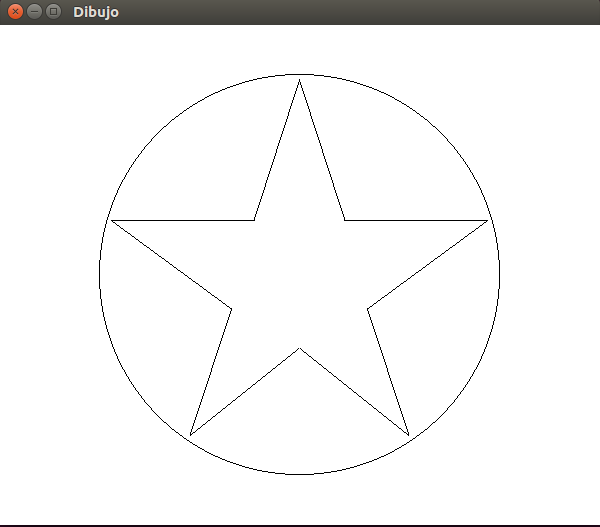
\includegraphics[scale = 0.5]{1.png}
  \caption{Resultados}
 \end{figure}
 
 \item \textbf{Figura 2: Sapito}
 
 \begin{lstlisting}
#include <iostream>
#include "primitivas.h"

using namespace std;

#define PI 3.14159265

GLsizei winWidth = 600, winHeight = 500;
Window window;


void init(void){
    glClearColor(1.0, 1.0, 1.0, 1.0);
    glMatrixMode(GL_PROJECTION);
    gluOrtho2D(0.0, 600.0, 0.0, 500.0);
}

void sapito(){
    Point centro;
    Point bocaDer;
    Point bocaIzq;
    Point bocaCurIzq;
    Point bocaCurDer;
    Point centroOjo;
    centro.x = winWidth / 2;
    centro.y = winHeight / 2;
    GLint radioCabezaY = 100;
    GLint radioCabezaX = 150;
    GLint radioOjo = 45;
    GLint radioOjito = 25;
    GLint distanciaAlOjo = 150;
    GLint anguloOjo = 80;
    GLint distanciaBoca = 110;
    GLint tamBoca = 90;
    GLint desplOjoX = distanciaAlOjo * sin(anguloOjo / 2 * PI / 180);
    GLint desplOjoY = distanciaAlOjo * cos(anguloOjo / 2 * PI / 180);

    Matrix cabeza = elipceMidPoint(centro, radioCabezaX, radioCabezaY, window);
    
    centroOjo.x = centro.x - desplOjoX;
    centroOjo.y = centro.y + desplOjoY;
    bocaDer.x = centroOjo.x;
    bocaDer.y = centroOjo.y - distanciaBoca;

    Matrix ojoDerecho = circleMidPoint(centroOjo, radioOjo, window);
    fillFigure(ojoDerecho, VERDE);
    glColor3f(0.0, 0.0, 0.0);
    Matrix ojitoDerecho = circleMidPoint(centroOjo, radioOjito, window);
    fillFigure(ojitoDerecho, BLANCO);

    centroOjo.x = centro.x + desplOjoX;
    centroOjo.y = centro.y + desplOjoY;
    bocaIzq.x = centroOjo.x;
    bocaIzq.y = centroOjo.y - distanciaBoca;

    glColor3f(0.0, 0.0, 0.0);
    Matrix ojoIzquierdo = circleMidPoint(centroOjo, radioOjo, window);
    fillFigure(ojoIzquierdo, VERDE);    
    glColor3f(0.0, 0.0, 0.0);
    Matrix ojitoIzquierdo = circleMidPoint(centroOjo, radioOjito, window);
    fillFigure(ojitoIzquierdo, BLANCO);
    fillFigure(cabeza, VERDE);

    glColor3f(0.0, 0.0, 0.0);
    
    bocaCurIzq.x = bocaIzq.x;
    bocaCurIzq.y = bocaIzq.y - tamBoca;
    bocaCurDer.x = bocaDer.x;
    bocaCurDer.y = bocaDer.y - tamBoca;
    Matrix lineaBoca = drawLineXnpio(bocaIzq, bocaDer, window);
    Matrix curvaBoca = bezier(bocaIzq, bocaDer, bocaCurIzq, bocaCurDer, window);
    Matrix boca = lineaBoca + curvaBoca;
    fillFigure(boca, BLANCO);
}

void display(){
    

    glClear(GL_COLOR_BUFFER_BIT);
    glColor3f(0.0, 0.0, 0.0);
    sapito();
    glFlush();

}

int main(int argc, char **argv){
    window.width = winWidth;
    window.height = winHeight;
    glutInit(&argc, argv);
    glutInitDisplayMode(GLUT_SINGLE | GLUT_RGB);
    glutInitWindowPosition(100,100);
    glutInitWindowSize(winWidth, winHeight);
    glutCreateWindow("Dibujo");

    init();
    glutDisplayFunc(display);
    glutMainLoop();
}
 \end{lstlisting}
 
 \begin{figure}[H]
  \centering
  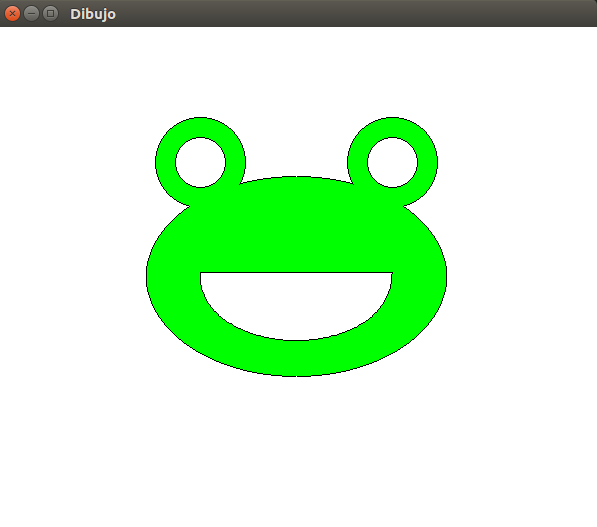
\includegraphics[scale = 0.5]{2.png}
  \caption{Resultados}
 \end{figure}





\end{enumerate}




\end{document}

